% Shared standalone design for the editable figure reconstructions.
\documentclass[tikz,border=5pt,10pt]{standalone}
\usepackage[T1]{fontenc}
\usepackage[utf8]{inputenc}
\usepackage{newpxtext,newpxmath}
\usepackage[scaled=.94]{sourcesanspro}
\usepackage{pgfplots}
\pgfplotsset{compat=1.18}
\usetikzlibrary{arrows.meta,calc,positioning,decorations.pathreplacing,
  decorations.markings,patterns,matrix,shapes.geometric,fit,backgrounds,
  intersections,angles,quotes}
\definecolor{ink}{HTML}{203746}
\definecolor{accent}{HTML}{146C78}
\definecolor{muted}{HTML}{667780}
\definecolor{signalred}{HTML}{B94B44}
\color{ink}
\tikzset{>=Latex,line width=.8pt,
  every node/.style={font=\small},
  axis/.style={->,draw=muted,line width=.5pt},
  guide/.style={draw=muted,dashed,line width=.45pt},
  curve/.style={draw=accent,line width=1pt},
  marker/.style={circle,fill=accent,inner sep=1.5pt},
  labelbox/.style={fill=white,inner sep=2pt}}

\begin{document}
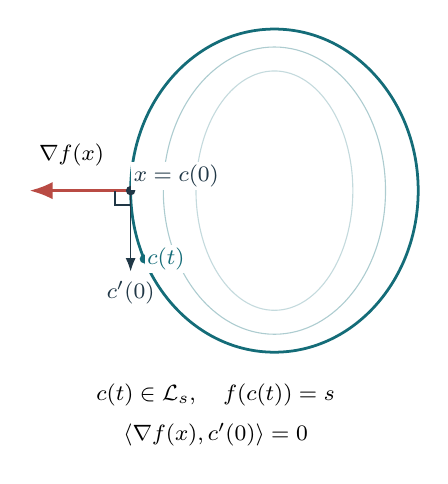
\begin{tikzpicture}[x=0.83cm,y=0.76cm,every node/.style={font=\footnotesize}]

\draw[accent!25] (3.4,2) ellipse (1.2 and 2);\draw[accent!35] (3.4,2) ellipse (1.7 and 2.4);
\draw[curve] (3.4,2) ellipse (2.2 and 2.7);
\coordinate (X) at (1.2,2);\draw[signalred,->,line width=1.2pt] (X)--(-.35,2) ;
\draw[->,ink] (X)--(1.2,.65) node[below] {$c'(0)$};\draw[ink] (1.2,1.76)--(.96,1.76)--(.96,2);
\fill[ink] (X) circle (1.7pt) node[above right,fill=white,inner sep=1pt] {$x=c(0)$};
\fill[accent] ({3.4+2.2*cos(205)},{2+2.7*sin(205)}) circle (1.6pt) node[right,fill=white,inner sep=1pt] {$c(t)$};
\node[anchor=west] at (-.35,2.6) {$\nabla f(x)$};

\node[align=center] at (2.5,-1.75) {$c(t)\in\mathcal L_s,\quad f(c(t))=s$\\[5pt]$\langle\nabla f(x),c'(0)\rangle=0$};
\end{tikzpicture}
\end{document}
